%%%%%%%%%%%%%%%%%%%%%%%%%%%%%%%%%%%%%%%%%%%%%%%%%%%%%%%%%%%%%%%%%%%%%%%%%%%%%%%%
% Template for USENIX papers.
%
% History:
%
% - TEMPLATE for Usenix papers, specifically to meet requirements of
%   USENIX '05. originally a template for producing IEEE-format
%   articles using LaTeX. written by Matthew Ward, CS Department,
%   Worcester Polytechnic Institute. adapted by David Beazley for his
%   excellent SWIG paper in Proceedings, Tcl 96. turned into a
%   smartass generic template by De Clarke, with thanks to both the
%   above pioneers. Use at your own risk. Complaints to /dev/null.
%   Make it two column with no page numbering, default is 10 point.
%
% - Munged by Fred Douglis <douglis@research.att.com> 10/97 to
%   separate the .sty file from the LaTeX source template, so that
%   people can more easily include the .sty file into an existing
%   document. Also changed to more closely follow the style guidelines
%   as represented by the Word sample file.
%
% - Note that since 2010, USENIX does not require endnotes. If you
%   want foot of page notes, don't include the endnotes package in the
%   usepackage command, below.
% - This version uses the latex2e styles, not the very ancient 2.09
%   stuff.
%
% - Updated July 2018: Text block size changed from 6.5" to 7"
%
% - Updated Dec 2018 for ATC'19:
%
%   * Revised text to pass HotCRP's auto-formatting check, with
%     hotcrp.settings.submission_form.body_font_size=10pt, and
%     hotcrp.settings.submission_form.line_height=12pt
%
%   * Switched from \endnote-s to \footnote-s to match Usenix's policy.
%
%   * \section* => \begin{abstract} ... \end{abstract}
%
%   * Make template self-contained in terms of bibtex entires, to allow
%     this file to be compiled. (And changing refs style to 'plain'.)
%
%   * Make template self-contained in terms of figures, to
%     allow this file to be compiled. 
%
%   * Added packages for hyperref, embedding fonts, and improving
%     appearance.
%   
%   * Removed outdated text.
%
%%%%%%%%%%%%%%%%%%%%%%%%%%%%%%%%%%%%%%%%%%%%%%%%%%%%%%%%%%%%%%%%%%%%%%%%%%%%%%%%

\documentclass[letterpaper,twocolumn,10pt]{article}
\usepackage{usenix2019_v3}

% to be able to draw some self-contained figs
\usepackage{tikz}
\usepackage{amsmath}

% inlined bib file
\usepackage{filecontents}

\usepackage{listings}
\usepackage{parcolumns}
\usepackage{graphicx}
\usepackage{caption}
\usepackage{subcaption}

%-------------------------------------------------------------------------------
\begin{filecontents}{\jobname.bib}
%-------------------------------------------------------------------------------
@book{silberschatz2018operating,
  title={Operating system principles},
  author={Silberschatz, Abraham and Galvin, Peter Baer and Gagne, Greg},
  year={2018},
  publisher={John Wiley \& Sons},
  edition={10}
}

\end{filecontents}

%-------------------------------------------------------------------------------
\begin{document}
%-------------------------------------------------------------------------------

%don't want date printed
\date{}

% make title bold and 14 pt font (Latex default is non-bold, 16 pt)
\title{\Large \bf TikTok: Kernel TOCTTOU Protection}

%for single author (just remove % characters)
\author{
{\rm Uro\v{s} Te\v{s}i\'{c}}\\
EPFL
\and
{\rm Mathias Payer}\\
EPFL
% copy the following lines to add more authors
% \and
% {\rm Name}\\
%Name Institution
} % end author

\maketitle

%-------------------------------------------------------------------------------
\begin{abstract}
%-------------------------------------------------------------------------------
Your abstract text goes here. Just a few facts. Whet our appetites.
Not more than 200 words, if possible, and preferably closer to 150.
\end{abstract}

% Talk about the system call filters and how they can be used for good
% Introduce the main problem - TOCTTOU
% Brag how our system is the best thing since sliced bread
\section{Introduction}
System call wrappers enable administrators to define system call execution policies. Such policies could prevent the execution of a system call based
on the ID of the call and its arguments. By setting only necessary access policies for all processes, administrators would reduce the damage in case that any of 
the processes get taken over by an adversary. 
Filtering could also restrict calls to the exploitable system calls. By excluding some combinations of arguments, the administrator could mitigate
certain vulnerabilities until a patch is available. Many embedded devices have binary-only drivers which prevent them from updating the kernel.
Malicious input filtering could be used as a permanent solution in those cases.
\\
\\
Unfortunately, system call wrappers suffer from a design flaw illustrated in \autoref{fig:tocttou}. System calls are independent of the filters, and execute after them. After a filter
reads the arguments and validates them, the system call reads them in the second time. In-between these two reads, the attacker could have swapped values,
leading to an execution of a forbidden call. This is called a \emph{time-of-check to time-of-use} attack (TOCTTOU). It is a consequence of a \emph{double-fetch}
from the userland and is notoriously hard to detect. Unlike other bugs, double-fetches are benign until the adversary decides to edit the arguments.
\\
\\
\begin{figure}[]
  \centering
  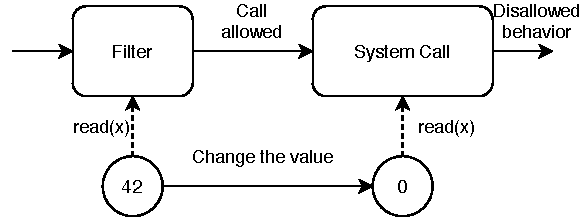
\includegraphics[width=.85\linewidth]{img/tocttou.pdf}
  \caption{Bypassing a system call filter using a TOCTTOU attack}
  \label{fig:tocttou}
\end{figure}
We present \emph{TikTok} - a mitigation for double-fetch bugs in Linux kernel. On every access
The contribution of this paper are:
\begin{itemize}
\item TikTok - a mitigation for time-of-check to time-of-use attacks on system call arguments
\item A technique to postpone the writes from userland
\item A technique to defer the writes from kernelland, while continuing normal kernel execution
\item A performance analysis of our system and its security guarantees
\end{itemize}

The rest of the paper is organized as follows: In \autoref{sec:background} we explain inter-process communication, paging, and double-fetch bugs. \autoref{}
% Cover the theory needed to understand how and why TikTok works
% 1) IPC - We need this to argue why the deadlocks are almost impossible
% 2) VM and Page Tables - Why it exists and how it works
% 3) x86 Page Tables - Continue the discussion from the previous section
% 4) Page faults - Explain how and why they happen.
\section{Background}

\label{sec:background}
\subsection{Interprocess Communication}

The two main types of communication between processes are: \emph{shared memory} and \emph{message passing}\cite{silberschatz2018operating}.
\\
\\
Shared memory relies on processes having a section of memory that both can access. Data tranfer is fast.
However, synchronization is problematic. Processes must monitor shared memory for changes, leading to unnecessary busy waiting.
\\
\\
Message passing consists of one process calling send, and another one calling receive to fetch the message.
Synchronization is guaranteed, with parties waiting for their calls to be server. However, unnecessary message 
copying can occur between processes on the same system.
\\
\\
Modern operating systems support both of these approaches. The downsides are usually offset by adding the 
bare minimum of the other approach (e.g. shared memory with semaphores, or message passing with shared buffers). 
However, only one of the methods is usually used between two processes. Communication by sending messages and writing
to the shared memory at the same time is quite rare.

\subsection{Virtual Memory and Page Tables} \label{sec:vm}

Operating systems (OS) provide an illusion that every process is executing alone on the processor. 
To accomplish this, OS needs to restore the program state on the context switch between two processes (e.g. CPU registers)
and to prevent processes from accessing each other's memory. Memory is protected by \emph{virtualization}. Processes use \emph{virtual
addresses} that get mapped to the actual (physical) addresses. When the OS moves data to a different physical address, the virtual
address refering to the data remains the same.
\\
\\
Virtual memory can be implemented by storing different processes' data at different offsets in physical memory, and limiting the
access to corresponding chunks of memory. Each process's memory chunk is called a segment and the implementation is called
\emph{segmented virtual memory}. The translation is accomplished by adding the offset to the virtual address. 
Considering that segments need to be continous, the free physical memory can be fragmented
such that the OS cannot find a part large enough to store a new process.
\\
\\
\begin{figure}

  \begin{subfigure}[]{.45\linewidth}
    \centering
    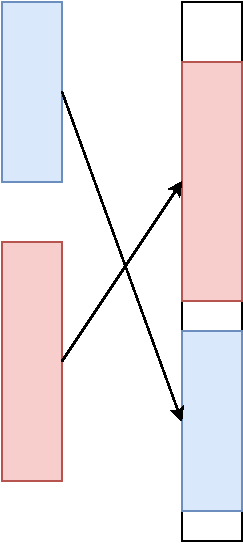
\includegraphics[width=.5\linewidth]{img/segmented.pdf}
    \caption{Segmented}
  \end{subfigure}
  \hfill
  \begin{subfigure}[]{.45\linewidth}
    \centering
    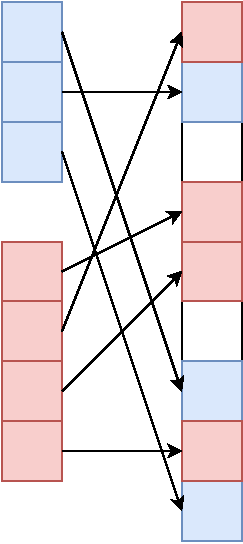
\includegraphics[width=.5\linewidth]{img/paged.pdf}
    \caption{Paged}
  \end{subfigure}

  \caption{Two virtual memory spaces mapped to physical memory using segmented and paged approaches}
\end{figure}

\emph{Paged virtual memory} is more flexible. The physical memory is partitioned into fixed-size pages (usually 4 kB).
A page in the virtual memory space gets mapped to the corresponding page in the physical memory. The mapping
function is defined for each process by a page-table. Page-tables store the number of the physical memory (\emph{page frame})
the virtual page points to. It also keeps the permissions the process has when accessing the page (\emph{read}, \emph{write},
\emph{execute}, \emph{user}, \emph{superuser}). In case of low memory, rarely accessed pages can be moved to the disk, and
replaced by immediately needed pages. This process is called \emph{swapping}. Similarly, when processing a file, pages don't
need to be loaded immediately, but on the first access (\emph{on-demand paging}). The \emph{present} bit is added to differentiate
between present and absent pages.
\\
\\
Virtual memory spaces are quite large today ($2^{64}$ bytes on a 64-bit processor). A table containing all one-to-one mappings would be
impossibly large to store. Page tables are therefore stored as trees with only the allocated memory being present (\autoref{fig:pagetable}).
However, instead of just reading the corresponding physical address on memory access, the processor now needs to perform a tree traversal.
Different bits in a virtual address correspond to the path the processor needs to take to
obtain the page frame number (e.g. the first 8 bits tell CPU which entry on the first level it needs to dereference). Considering that this
process needs to be fast, it is implemented in hardware by the \emph{memory management unit} (MMU). Reading the page table from memory is
slow, so a small cache is added to the MMU to store frequently accessed page entries - \emph{translation-lookaside buffer} (TLB). On modern
processors TLB consists of several levels, and can even be backed by an another MMU cache. 

\subsection{x86-64 Page Tables}

\begin{figure}[]
  \centering
  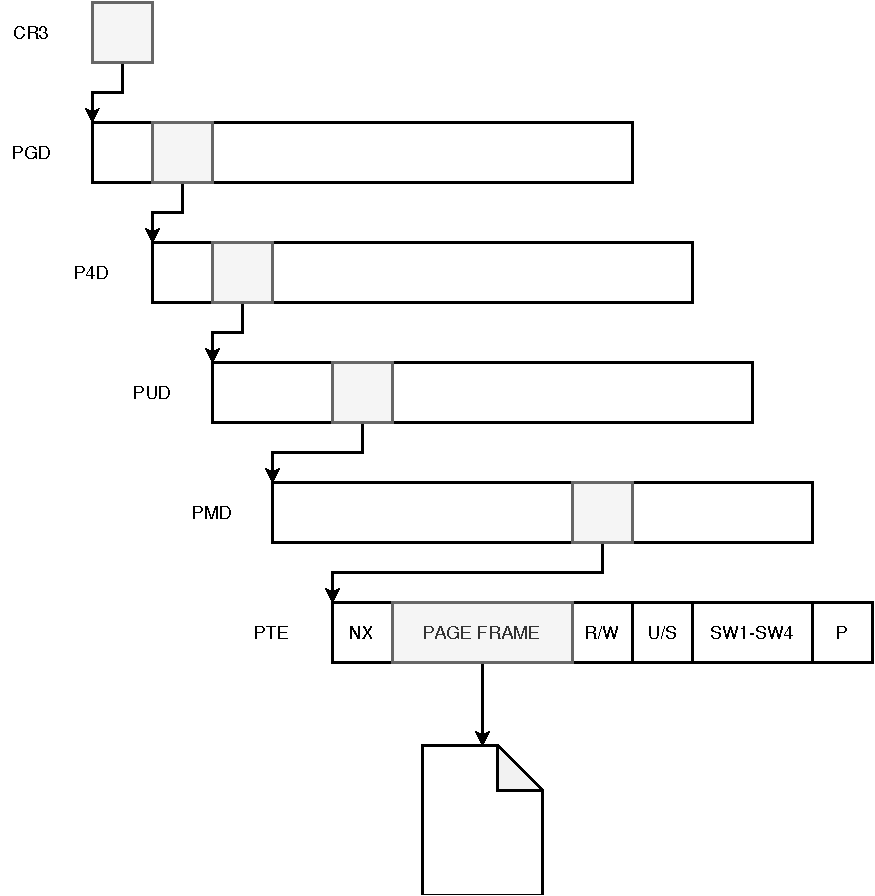
\includegraphics[width = .35 \textwidth]{img/pagetable.pdf}
  \caption{Page Table Structure on x86. Only relevant data has been included.}
  \label{fig:pagetable}
\end{figure}
x86-64 architecture officially supports paged virtual memory model with 5 levels of page tables (\autoref{fig:pagetable}):
\begin{description}
    \item[PGD] Page Global Directory
    \item[P4D] Page Fourth-level Directory
    \item[PUD] Page Upper Directory
    \item[PMD] Page Middle Directory
    \item[PTE] Page Table Entry
\end{description}

Every level corresponds to 8 bits in the virtual address, with the remaining 12 bits identifying the offset of the byte in the actual page frame.
Page table entry includes the following information:
\begin{description}
    \item[Present bit (\textbf{P})] denotes if the page is present in memory
    \item[Read/Write bit (\textbf{R/W})] denotes if the page is writable, or only readable
    \item[User/Superuser bit (\textbf{U/S})] denotes if the page can be accessed by the user, or only by the superuser
    \item[Not Executable bit (\textbf{NX})] denotes if the code stored on the page can be executed
    \item[Page Frame Number] denotes the page frame the entry points to
    \item[\textbf{SW1-SW4}] Four bits free for the OS to use
\end{description}

\subsection{Page-Faults}
On an invalid access (e.g. wrong permissions, page not present) the MMU will trigger a page-fault. The fault is a type of a synchronous
interrupt which executes in the context of the faulting (accessing) thread. The page-fault handler loads an absent page from the disk.
In case of a write to a temporarily shared page, it creates an independent copy of the page (\emph{copy-on-write}). In case of a
permission violation the page-fault handler kills the thread. After the fault finishes executing, the faulting instruction is reexecuted. 
\\
\\
With the advent of cloud computing, userland page-fault handling has been added to the Linux kernel. Users can define their own routines
to page in swapped data. This is particularly useful on computer farms when migrating virtual machines between physical nodes. One only needs
to migrate the code that is executing. Accesses to the unmigrated memory will be passed to the userland page-fault handler. It will then
fetch them over the network and continue the execution.

\subsection{Copy-from-User and Copy-to-User}
Linux uses swapping only for user memory. When executing in kernel context, kernel memory is mapped and present. A page fault on kernel
memory access is therefore always fatal. However, the kernel needs to access user memory, which can cause a page-fault. User memory is
also limited to the lower half of virtual memory space, requiring checks on every access.
\\
\\
To force and encapsulate those checks Linux provides functions and macros for user-memory access from the kernel-space. A page-fault
generated in them is handled like a fault in the user process which called the executing system call.
\\
\\
The interface for communication with userspace:
\begin{itemize}
    \item[] \texttt{copy\_(from/to)\_user}
    \item[] \texttt{\_\_copy\_(from/to)\_user}
    \item[] \texttt{(get/put)\_user}
    \item[] \texttt{\_\_(get/put)\_user}
    \item[] \texttt{user\_strcpy}
    \item[] \texttt{user\_strlen}
\end{itemize}
\bigskip
BSD also provides a similar interface using \texttt{copy\_in} and \texttt{copy\_out} functions.

\subsection{Double Fetch Bugs}

Double-fetch bugs occur when

\label{sec:doublefetch}

\section{Design}
\label{sec:design}
In this section we describe a high-level overview of TikTok. We start with the security model in \autoref{subsec:secmodel}.
Afterward we describe how TikTok protects system call arguments from userland (\autoref{subsec:userland}) and kernelland 
(\autoref{subsec:kernelland}) writes

\subsection{The Security Model}
\label{subsec:secmodel}
The administrator has set up DAC preventing the adversary from accessing files mapping to physical devices.
They also control which file-systems are mounted on the machine and have disabled userland page-fault handling.
\\
\\
The adversary has access to a user account on a target machine. They can execute arbitrary code (including system call)
and want to obtain root access by triggering a TOCTTOU bug in the kernel.

\subsection{Protecting System Call Arguments from Writes by the User}
\label{subsec:userland}
\begin{figure}[]
  \centering
  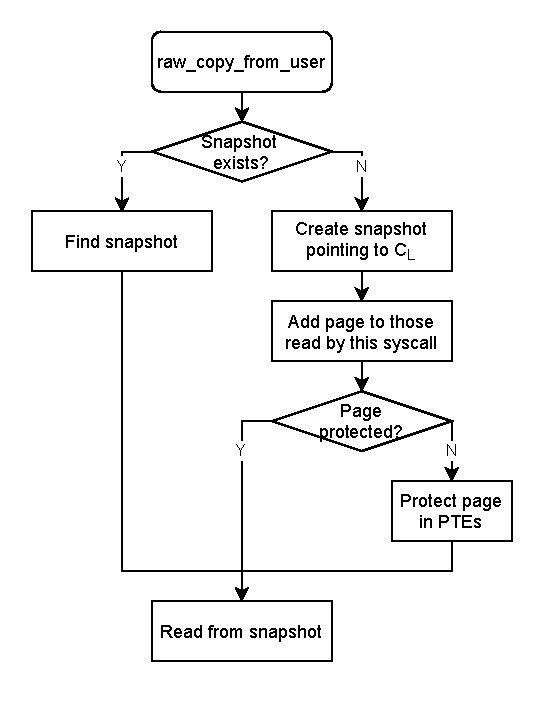
\includegraphics[width = .45 \textwidth]{img/copy_from_user.pdf}
  \caption{\texttt{copy\_from\_user} marks both the file and the pages before reading in the data}
  \label{fig:pagetable}
\end{figure}

System calls access the user memory via \texttt{copy\_from\_user} and its variants. When that happens, 
TikTok \emph{marks} the entire page storing the argument as \emph{read-only} in all virtual memory spaces 
mapping it (\autoref{fig:copyfromuser}). Multiple system calls can mark a page at the same time. Marking a page does not affect reads
from userspace in any way. When all the system calls that use the page finish executing, the page is \emph{unmarked} - its
previous permissions are restored.
\\
\\
Writes to the marked pages will trigger a page-fault (\autoref{fig:pagefault}). In the page-fault handler we intercept these writes 
and make them wait for the page to get unmarked. The faulting thread attempts to perform the
write again.

\begin{figure}[]
  \centering
  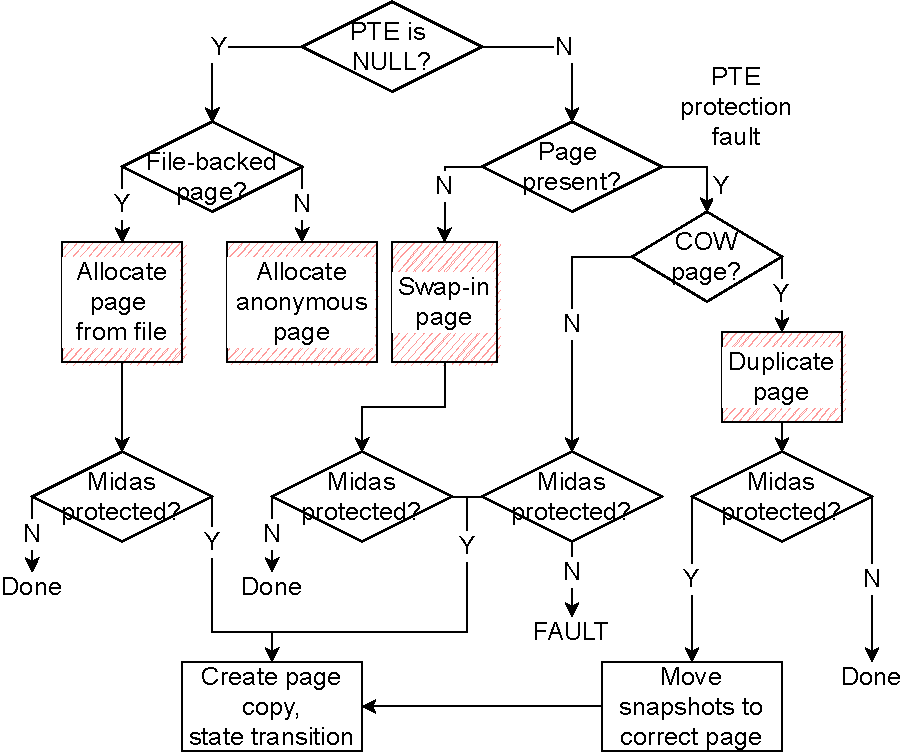
\includegraphics{img/pagefault.pdf}
  \caption{TikTok's handling of the writes to a marked page}
  \label{fig:pagefault}
\end{figure}

\subsection{Protecting System Call Aguments from Writes by the Kernel}
\label{subsec:kernelland}
\begin{figure}[]
  \centering
  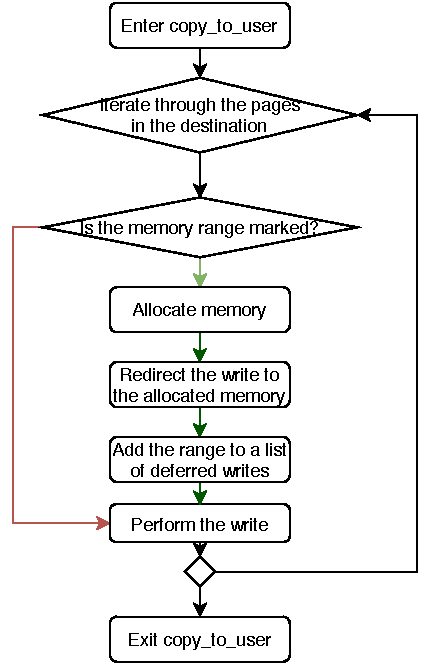
\includegraphics[width = .30 \textwidth]{img/copy_to_user.pdf}
  \caption{\texttt{copy\_to\_user} defers the writes from kernel until the end of the system call}
  \label{fig:pagetable}
\end{figure}

Watson mentions in \cite{watson} that the system call wrappers he analyzed don't handle writes from kernelspace
properly. Unlike those solutions, TikTok doesn't copy arguments to separate pages, leading to complex redirection 
of userspace pointers. This unables us just to defer the writes until it is safe to perform them.
\\
\\
However, deferring kernel writes the same way as user writes would lead to deadlocks. System call \texttt{rt\_sigaction}
needs to write to a page it previously marked. Pausing execution would leave the thread in a state where it is waiting for itself
to exit unmark the page. Temporarily unmarking the page would enable an adversary to edit arbitrary data on it.
\\
\\
Allowing the writes for the kernel is not an option. The adversary could abuse this to change the marked memory. 
They would execute a read system call into the marked page. System calls execute in the kernel context and would 
be able to bypass protection. The read system call would then write arbitrary data into the protected area.
\\
\\
Our solution is based on the fact that we already provide partial checkpointing of the system call's view of RAM.
During its execution, the system call can only see the state of the memory as it was at the beginning of the call.
All writes from userspace become visible only when the call has finished execution. TikTok extends this policy to 
writes from kernelspace. Considering that we need to continue execution after a write to a marked page, we buffer 
all the writes until the system call finish. At that point we unmark the pages and allow them to proceed normally.

\subsection{Ignored System Calls}
\label{subsec:ignoredcalls}

Some system calls (e.g. \texttt{pollfd} and \texttt{futex}) rely on writes from userland for some of their functionality. Marking their arguments
would lead to deadlocks, so they are ignored. Considering that attacking these system calls would to expected behavior, the authors
don't consider this a deficiency.
\\
\\
Other system calls can be ignored as an optimization. Any unformatted data that is passed to the kernel doesn't need
to be marked by TikTok. Overwriting this data is equivalent to passing different data to the call. Considering
that the write call takes unformatted data as one of its arguments, this frequently called interface doesn't need to
be protected.

\subsection{Two Axes of the Linux Memory}

Memory in Linux can be \emph{file-backed} and \emph{anonymous}. File-backed pages have map to a corresponding file. 
Anonymous pages don't have a backing file (e.g. stack and heap).
\\
\\
Another classification is based on privacy: \emph{private} and \emph{shared}. Private memory is part of only one virtual memory space.
This memory space can be accessed by multiple threads in a process, but no threads outside the process have access.
Shared memory can be accessed by multiple processes.
\\
\\
\begin{table}[]
  \begin{tabular}{|l|l|l|}
  \hline
          & Anonymous                            & File-backed                           \\ \hline
  Private & /                                    & Copy-on-write                         \\ \hline
  Shared  & Inherited by fork                    & Can be (un)mapped at any time         \\ \hline
  \end{tabular}
  \caption{Properties of the different types of memory in Linux}
  \label{tab:memory}
\end{table}
Unlike private memory and shared anonymous memory, shared file-backed memory can be mapped and unmapped at will (\autoref{tab:memory}). It 
also preserves its state. This enables an adversary to map a marked page as writable and edit it. 
TikTok intercepts mapping of memory and checks the page frames being mapped. The pages are then mapped
with appropriate permissions into the virtual memory space.
\\
\\
Devices are treated as files in Linux and can be memory mapped. However, hardware may change its registers at will.
There are no conceivable ways from protecting from TOCTTOU attacks if the adversary stores his arguments in device
mapped memory. Considering that mapping device memory to userland is considered bad practice, we rely on \emph{Descretionary
Access Control} (\textbf{DAC}) to prevent users from mapping devices in the first place.

\subsection{File Writes}
\label{subsec:filewrites}
Files in Linux can be accessed in two ways:
\begin{itemize}
    \item by mapping the file to memory
    \item by using system calls to modify the file (e.g. \texttt{write})
\end{itemize}

Watson has noticed that protected file-backed pages could still be edited by a \texttt{write} call. TikTok prevents this attacks
by pausing the write to the corresponding file as long as it has any marked mapped pages.

\subsection{TikTok Deadlocks}
\label{subsec:deadlocks}
TikTok adds additional synchronization points to multithreaded programs. It is possible for these points to introduce 
previously non-existant deadlocks to programs. However, deadlocking threads would need to communicate using both 
shared memory (for TikTok to stop one of them) and message passing system calls (for TikTok to mark memory).


\begin{figure}
  \centering
  \begin{subfigure}[b]{0.45\linewidth}
  \begin{minipage}{\linewidth}
  \begin{lstlisting}
  1: S(A,T1);  
  \end{lstlisting}
  \end{minipage}
  \caption{Thread 1}
  \end{subfigure}
  \hfill
  \begin{subfigure}[b]{0.45\linewidth}
  \begin{minipage}{\linewidth}
  \begin{lstlisting}
  2: write(A);
  3: unblock_S(T2);
  \end{lstlisting}  
  \end{minipage}
  \caption{Thread 2}
  \end{subfigure}
  \caption{Executing instructions in the specified order causes a deadlock with TikTok}
  \label{fig:deadlock}
\end{figure}


\autoref{fig:deadlock} shows an example of a such communication pattern. Thread 1 enter the system call S and marks the shared page A (\textbf{1}).
The system call S blocks untill a corresponding call \texttt{unblock\_S} is called in Thread 2 (\textbf(3)). While the page \texttt{A} is still marked, Thread 2
attempts to write to it, causing it to wait for \texttt{S} to finish (\textbf{2}).
This situation is perculiar:
\begin{enumerate}
    \item The page \textbf{A} is shared between Thread 1 and Thread 2
    \item Access to page \textbf{A} isn't protected by a mutex, or a semaphore
    \item System call \textbf{S} is a blocking system call that receives a signal from another thread
    \item System call \textbf{S} reads its arguments from the page \textbf{A}
    \item Thread 2 needs to write to the same page where the arguments for \textbf{S} are stored (page \textbf{A})
    \item Even though Threads 1 and 2 can communicate using shared memory, Thread 1 needs to also invoke \textbf{S}
\end{enumerate}

While a a synchronization call (locking or signaling) would be a good candidate for S, they are lightweight and their arguments
are passed in registers, not in memory. A message-passing call fits the description better. Data from page A would need to be marked,
as it is read by the call. Message-passing can also be synchronous, requiring the other thread to receive the message before proceeding.
However, why would two threads communicate using both message passing and shared memory?
\\
\\
While it is possible to create deadlocking sequences, they require mixing different inter-process communication
paradigms for the same data. During testing we haven't encountered a single permanent deadlock.
\\
\\
Similar sequences can be constructed using the write system call protection presented in \autoref{sec:filewrites}. The same argument
can be applied in that case - the program would need to write to the same data to the file using both memory mapping and a system call. We
haven't encountered such a problem.


\section{Implementation}

\subsection{Storing the Page Frame Information}

Linux divides physical memory into page frames. Each page frame is represented by \texttt{struct page}. Considering that that this structure
is replicated millions of times, every additional field has a tremendeous impact on memory consumption. What's even worse, the cost would not
be constant, but linear. Systems with more memory would also waste proportionally more RAM.
\\
\\
To keep the memory consumption low, TikTok uses a single bit in \texttt{struct page} to mark page frames. Considering that the prototype is implemented on x86-64,
we decided to use one of the flag bits for this purpose. Architectures which have fewer flag bits (such as x86) could decide to recycle some of
the bits used by other features (e.g. Kernel Shared Memory). The marking information is stored separately - in a hashmap.
Access to these entries is protected by separate mutexes.

\subsection{Keeping Track of Marked Pages}

When TikTok marks a page on x86-64, it uses an extra bit in the PTE to differentiate it from non-marked PTEs. Another bit is used to remember old R/W permission.
Depending on which exact bits are used, some kernel features may need to be disabled. In the prototype TikTok shares one of the page table bits with page tracking.

\subsection{Implementing TikTok on Other Architectures}



\section{Related Work}

Literature relating to TikTok can be broadly divided in 2 groups. The first group are system call wrappers and filters whose main vulnerability TikTok is mitigating.
The second one are the mitigations and solutions for double-fetches, which are a superclass of TOCTTOU bugs. We discuss both groups in this section and describe the
benefits TikTok brings to the first group, and the advantages over the second group.

\subsection{System Call Wrappers and Filters}

Watson in \cite{watson} scrutinized the security of many system call wrappers. Not only that he found that all of them were insecure, Watson described the different
types of TOCTTOU bugs and discussed potential fixes.
In a short paragraph he mentiones that Pawel Dawidek, the creator of CerbNG \cite{cerbng}, has experimented with marking arguments read-only. CerbNG was an early 
attempt at filtering system calls for BSD that used copying to protect the arguments. To our knowledge nothing came out of those experiments. 
\\
\\
Watson briefly discusses problems the memory marking systems need to solve: 
\begin{itemize}
    \item unnecessary page-faults
    \item bypassing memory marking using IO system calls
    \item mapping shared memory late
    \item handling system calls that write to memory correctly
\end{itemize}

TikTok addresses all of these problems. Unnecessary page-faults are rare and they are used to make the offending threads wait for unmarking. After the page has been unmarked,
the write proceeds without any consequences. Write system call does not proceed until there are no marked pages of the file. If needed, pages are marked when they are mapped. 
TikTok also postpones all writes to marked pages coming from kernelspace, while allowing the system calls to execute correctly.
\\
\\
Modern system call wrappers can be classified in two groups, based on how they approach the TOCTTOU attack. The first group eliminates all functionality vulnerable to the attack.
Linux's \emph{SecComp} and \emph{eBPF} belong to this group. The second group moves the filter checks deeper into the system calls, eliminating the need to read the arguments
twice. \emph{Landlock Linux} and Google's \emph{KPSI} embrace this technique.

\subsubsection{Partial Solutions}
SecComp uses \emph{Berekley Packet Filter} (BPF) to provide small, programmable filters that execute before the system call. Based on the values in registers, Linux can decide whether
to allow, or to prevent a system call. However, BPF cannot dereference pointers because an adversary would by able to bypass those checks due to the TOCTTOU. 
\emph{Extended Barekley Packet Filter} (eBPF) provides larger filters which can also dereference user pointers. However, eBPF cannot be used for security purposes - it cannot stop
system calls from executing. EBPF is completely read-only and can only be used for tracing.
\\
\\
\subsubsection{LSM-based Solutions}
Landlock and KPSI use \emph{Linux Security Module}\cite{lsm} (LSM) hooks to call filter checks after the arguments have already been copied into the kernel. LSM hooks have been imagined
as a set of places where pointers to functions can be called to perform an arbitrary check. Execution proceeds only if the execution has been successful. Different security modules
can provide different hooks to provide different guarantees (e.g. \emph{SELinux} and \emph{AppArmor}).
\\
\\
Both Landlock and KPSI attach eBPF filters to hooks, allowing users to provide custom rules for system calls. For this solution to work everywhere for perfect syscall filtering, 
LSM hooks would need to be manually added to all Linux drivers and ioctls. Unfortunately, this is highly impractical and requires a considerable effort from a large group of developers.
TikTok is a generic solution that doesn't require modifying the drivers, nor the use of LSM hooks. Once it is deployed, double-fetches are eliminated from all the drivers.

\subsection{Double-Fetch Solutions}

Wang et al showed in \cite{wang07} showed that double-fetches appear not only in kernels, but wherever there is a trust boundary to cross (e.g. kernel -- hypervisor).
By analyzing reported CVEs they classified double-fetches in several groups based on the code context and their effects (i.e. severity). Another interesting point they raised
is that double-fetches can appear in valid code as a result of compiler optimizations.
\\
\\

\subsubsection{Static Analysis Work}
Static analysis techniques analyze the source code to find double-fetch bugs. Wang et al \cite{usenixwang07} used pattern matching to find potential double-fetches. However, 
this technique results in a large number of false positives that need to be pruned manually. Xu et al's \cite{xu18} proposed Deadline - an improved technique that is
able to automatically determine if double-fetches result in a potential vulnerability. Instead of relying of pattern matching they compiled the code into the intermediate representation
and symbolically executed the code.
\\
\\
While static analysis techniques have the benefits of being able to find the bugs in code that we cannot actually run (e.g. we are missing hardware to test the drivers), it can only 
detect the bug in the best case. The developers still need to fix it. In case of syscall wrappers, we are aware that the bug is present, but it is there by design. TikTok can prevent
double-fetches in cases like this, or when we aren't even aware that they are present (e.g. compiler introduced).
\\
\\

\subsubsection{Dynamic Analysis Work}
Google Project Zero's Bochspwn \cite{bochspwn} was an early work on fuzzing kernel code inside an emulator to detect double-fetches. It found an quite a large number of bugs in the Windows
kernel. It works on binaries and doesn't require access to the source code. However, it is limited to the detection of double-fetches. All found cases need to be manually triaged and fixed
by developers. For a double-fetch to be detected it needs to be executed, limiting this techniques to the core kernel and to the drivers with the available hardware.
\\
\\
A big leap in dynamic analysis techniques has been presented by Schwartz et al \cite{schwarz18}. While Bochspwn reliesThe first part of the paper introduces DECAF - a framework that uses side-channel attacks to
create a fuzzing oracle for double-fetch bugs. Much like Bochspwn, this technique can detect double-fetches invisible to static analysis, but is orders of magnitude faster. DECAF also prunes
false positives by trying to automatically exploit double-fetches it has detected.
\\
\\
However, they also discuss a real-time mitigation technique for these bugs - DropIt. Unfortunately, DropIt relies 
on Intel's Transactional Memory Extensition (TSX). TSX introduces limits to the size of the code that can be protected and instructions that can be used inside the protected section. Because
of its use in side-channel attacks, both Intel and Linux have dropped supprot for TSX. As a consequence, this technique doesn't work anymore. TikTok has none of the limitations of DropIt and
relies only on page access control for protection - a technique which has been already been present for several decades.


%-------------------------------------------------------------------------------
\section*{Acknowledgments}
%-------------------------------------------------------------------------------

Thanks, mom!

%-------------------------------------------------------------------------------
\section*{Availability}
%-------------------------------------------------------------------------------

The source code of TikTok is available at LINK. It has been released under the
GNU Public Licence.

%-------------------------------------------------------------------------------
\bibliographystyle{plain}
\bibliography{\jobname}

%%%%%%%%%%%%%%%%%%%%%%%%%%%%%%%%%%%%%%%%%%%%%%%%%%%%%%%%%%%%%%%%%%%%%%%%%%%%%%%%
\end{document}
%%%%%%%%%%%%%%%%%%%%%%%%%%%%%%%%%%%%%%%%%%%%%%%%%%%%%%%%%%%%%%%%%%%%%%%%%%%%%%%%

%%  LocalWords:  endnotes includegraphics fread ptr nobj noindent
%%  LocalWords:  pdflatex acks
